\documentclass[a4paper, 12pt, one column]{article}

%% Language and font encodings. This says how to do hyphenation on end of lines.
\usepackage[english]{babel}
\usepackage[utf8x]{inputenc}
\usepackage[T1]{fontenc}

%% Sets page size and margins. You can edit this to your liking
\usepackage[top=1.3cm, bottom=2.0cm, outer=2.5cm, inner=2.5cm, heightrounded,
marginparwidth=1.5cm, marginparsep=0.4cm, margin=2.5cm]{geometry}

%% Useful packages
\usepackage{graphicx} %allows you to use jpg or png images. PDF is still recommended
\usepackage[colorlinks=False]{hyperref} % add links inside PDF files
\usepackage{amsmath}  % Math fonts
\usepackage{amsfonts} %
\usepackage{amssymb}  %
\usepackage{array} % enable column sizing
\usepackage[section]{placeins} %prevents figure jumping to end of document
\usepackage{float}
\usepackage[normalem]{ulem}

%% Citation package
\usepackage[authoryear]{natbib}
\bibliographystyle{abbrvnat}
\setcitestyle{authoryear,open={(},close={)}}



\begin{document}

\begin{figure}
		
\includegraphics[width=\linewidth]{Images/logo.jpg}	
\end{figure}
    
\title{NavUP System}
\author{
				Claassen Charles u15216498]\\
                Daubinet Jordan u15260870\\
                Kanda Madimba u17289077\\
                Ngobale Nathan u15110045\\
                Olwage Dedré u15015239\\
                Sargeant Lucian u15225560\\
                Tshela Bongani u14134790\\
        }
        
\maketitle
	\begin{center}
			\url{https://github.com/ProBlack95/SE-Go-Team}	
	\end{center}
	\newpage
    
\tableofcontents
\newpage

\section{Introduction}
We have been tasked with drafting the Architectural Requirements Specifications and Design for the NavUP system. This document contains the design of the Users, Data, Navigation and Fitness modules as well as a broad overview of the entire system.

\section{External Requirements For The System}
\subsection{Hardware Interface Requirements}
The main hardware interface requirements for the system extend to the need for a central server which will store user and map data. This server will interface with the Users, Data and GIS module providing data for various functions of these modules that require the retrieval of data. The NavUP system will have an Android and iOS front-end which means the mobile device, on which the NavUP system is running, will act as an interface between the user and the abstract software system. These devices themselves are required to have certain hardware based specifications these being: a WiFi chip for connection to the UP network providing Internet access and connection based position determination, a GPS chip for satellite based communication and triangulation and an accelerometer in order to track motion and in so doing record steps of the user.  
\subsection{Software Interface Requirements}
The system will need to be able to create communication interfaces between the operating systems that are running on the various devices present in the system. These operating systems include Android, iOS, windows Server, Linux and various less well know occurrences perhaps running on satellites or WiFi routers. These communication pathways will need to allow for transfer of data between devices running different operating systems. On a more abstract level, there will need to be additional code to allow for the integration of various APIs into the system. 
\subsection{User Interface Requirements}
The system will incorporate an Android, iOS and web-based front-end for the user to interact with. The user interface for the system should provide an easy means for the user to select a destination they would like to travel to and be presented with a number of possible routes. This could be accomplished by immediately presenting the user with a map of campus localised to their current position. A search bar along the top will allow the user to search for a destination from which they’ll be shown a zoomed out view of campus with the possible routes highlighted on the map. They would then be able to select a route and would be presented with screen or voice based, turn by turn instructions to reach their desired destination. An additional menu button could bring up options to set the user’s route preference or access their saved routes. The interface can also provide text-to-speech functionality for users with disabilities.
\newpage
\subsection{Communication Interface Requirements}
There are multiple devices within the NavUP system and as a result communication between them is imperative. In terms of the main function of the system of finding a route, the navigation module will create a GIS request that will be sent to the GIS module which will in turn use the required communication protocols to access and retrieve map data from the GIS database. A GIS request could also be for utilising the device’s GPS chip and communicating with a satellite to determine device position. Alternatively the WiFi chip could be used and based on its communication, via network protocols, with nodes in the UP network, the device position could theoretically be determined. For the less direct and more integrated functions of the system registered user data will need to accessed from the various servers and databases and this will be accomplished via the appropriate network protocols. 
    
\section{Data Module}
	The Data module handles the interactions with the users and the server. Users from different platforms connect to the Access Channel which interacts which interacts with the upstream Manager. The up-stream Manager is the gateway for user requests and responses from the down-stream Manager. The down-stream manager gives all up-stream requests to the server and sends all server responses to the up-stream Manager. The Design patterns which are integrated into the Data Module are: Singleton, chain of responsibility, template, iterator and interface. the Singleton design pattern ensures only one UpStreamManager, DownStreamManager and AccessChannel exist at any time. The chain of responsibility design pattern is used to pass requests up from the user platforms to the server and to pass stream objects from the server to the user platforms. The template design pattern is used to implement different handling methods for the requests of the different concrete platforms used to connect to the access channel. The iterator design pattern is used for the server to iterate through users when concurrently sending multiple stream objects to different users. The interface design pattern is used to implement how the server acts as an interface for all subsystems.
    
        
\subsection{Design Constraints}
Some design constraints for the data module include:
  \begin{itemize}

      \item The correct data types for information to be entered into the system database need to be carefully chosen. 
    Data types need to fit accordingly as to not watse overall system storage and downgrade the systems performance.

      \item The system server needs to be equipped with a quality processor in order to process mass amounts of upstream and downstram data at the same time.
    Failure to implement a quality processor, might lead to the system crashing under the pressure of mass amounts of requests from users.

    \item The server hardware need be equipped with the correct and necessary security measures.
    Failure to equip the server with the correct and necessary security measures might lead to the system database being at risk,
    which can lead to sensitive user information being at risk for theft or even loss.

  \end{itemize}
  

\subsection{Technology Choices}

For this module to work effectivley, we must me able to query and add users details to the database. We will use SQL for databases for all the platforms. PHP will help in retrieving data (Mostly for Web). The SQLiteOpenHelper import (IOS/Android) will help us use SQL query and add fuctions for both platforms.
For the user Interface and navigation through pages we will use Android studio and Xcode for IOS or we could use a cross platform tool for all the platforms(e.g PhoneGap). 

\begin{center}
\subsection{Class Diagram}
        \includegraphics[width=\linewidth,angle=90,scale=1.3]{Images/DataModule/DataModuleClassDiagram.png}
        \begin{figure}[h]
            \caption{Data Module Class Diagram.}
        \end{figure}
        
\subsection{Use Case Diagram}
        \includegraphics[width=\linewidth,angle=90,scale=1.3]{Images/DataModule/DataModuleUseCaseDiagram.png}
        \begin{figure}[h]
            \caption{Data Module Use Case Diagram.}
        \end{figure}
        
\subsection{System Activity Diagram}
        \includegraphics[width=\linewidth,angle=90,scale=1.3]{Images/DataModule/DataModuleSystemActivityDiagram.png}
        \begin{figure}[h]
            \caption{Data Module Use Case Diagram.}
        \end{figure}
\end{center}
        
\section{Navigation Module}
The Navigation module is the functional core of the system providing all of the routing functionality. Different types of routes are available for calculation, these being: the shortest route, the simplest route, the most popular route or a user defined route. Each of these choices will, in the end produce a route, the only difference between them being the process or algorithm used in producing this route. As a result the module has been modeled using a strategy design pattern to separate the different strategies or algorithms into their own classes reducing coupling but maintaining cohesion.

\subsection{Design Constraints}
\begin{itemize}

      \item The system using the Navigation module must have WiFi support with an intenet connection to be able to get real time updates of the map and route changes.
      \item The system should also include suppot for a GIS to be able to find the user's current location at all times.
       \item The system should also include a monitor to display the mapp and route information to the user and the system will also require a processor strong enough to calculate the different routes to the user's selected destination.
        \item The Navigation module should also be able to record the route the user is taking or a route the userr has chosen and send that information to the data module to store the route as a preference.
      
  \end{itemize}

\subsection{Technology Choices}
Leaflet is an open-source JavaScript library that provides mapping functions for mobile developers. It runs efficiently on all major mobile and desktop platforms and therefore satisfies our requirement of the NavUP system needing to have Android, iOS and a web-based frontend. Leaflet can work with custom GIS data so will allow for the use of our provided GIS mapping of the University of Pretoria’s campus. The API at a basic level is mainly for displaying map data however there are a number of plugins available to expand the functionality. One of these is called Leaflet Routing Machine and provides a graphical extension to leaflet, displaying routes between a start and end point. Leaflet routing machine provides additional functionality for backend routing engines, one of these being OSRM (Open Source Routing Machine). OSRM uses extremely fast methods for shortest path routing and provides turn by turn navigation instructions to the user. These three technologies already interface with one another, are all open source and satisfy most of the constraints of the NavUP Navigation module. Additional implementation could ensure that the technologies integrate well into the NavUP system.

\begin{center}
\subsection{Class Diagram}
        \includegraphics[width=\linewidth,angle=90,scale=1.3]{Images/NavigationModule/Navigation_Class_Diagram_Final_.png}
        \begin{figure}[h]
            \caption{Navigation Module Class Diagram.}
        \end{figure}
        
\subsection{Use Case Diagram}
        \includegraphics[width=\linewidth,scale=2]{Images/NavigationModule/Navigation_Use_Case_Diagram.png}
        \begin{figure}[h]
            \caption{Navigation Module Use Case Diagram.}
        \end{figure}
        
\subsection{Activity Diagram}
        \includegraphics[width=\linewidth,angle=90,scale=1.4]{Images/NavigationModule/Navigation_Activity_Diagram.png}
        \begin{figure}[h]
            \caption{Navigation Activity Diagram.}
        \end{figure}
        
\end{center}
        
\section{User Module}

The user management module is responsible for maintaining information about the registered users of the system, including the authority levels of each user.

The bridge design pattern is used when we need to decouple an abstraction from its implementation so that the two can vary independently. The pattern has the User class (Interface) which acts as a bridge which makes the functionality of the Guest and RegUser classes(concrete classes) independent from interface implementer classes. Now the Guest and RegUser type classes can be altered structurally without affecting each other.

The builder design pattern builds a complex object using simple objects and using a step by step approach. It provides one of the best ways to build an object. A Builder class builds the final object step by step so is independent of other objects. 

Singleton makes sure that only a single Admin(User) object is instantiated for each user. The Admin class provides a way to access its only object which can be accessed directly without need to instantiate the object of the class.

\subsection{Design Constraints}
\begin{itemize}
	\item Strict forms must be used with data verification to validate entered data and avoid attacks such as SQL injections.
    \item Careful procedures must be put in place to ensure that only designated individuals may register as admin users.
    \item Users must each have a unique identifier ID which could be determined by a combination of email address with another field.
\end{itemize}
\subsection{Technology Choices}
For this module to work effectively, we must be able to query and add user's details to the database. We will use SQL for databases for all the platforms. PHP will help in retrieving data (Mostly for Web). The SQLiteOpenHelper import (IOS/Android) will help us use SQL query and add functions for both platforms.
For the user Interface and navigation through pages we will use Android studio and Xcode for IOS or we could use a cross platform tool for all the platforms(e.g PhoneGap). 

\begin{center}
\subsection{Class Diagram}
        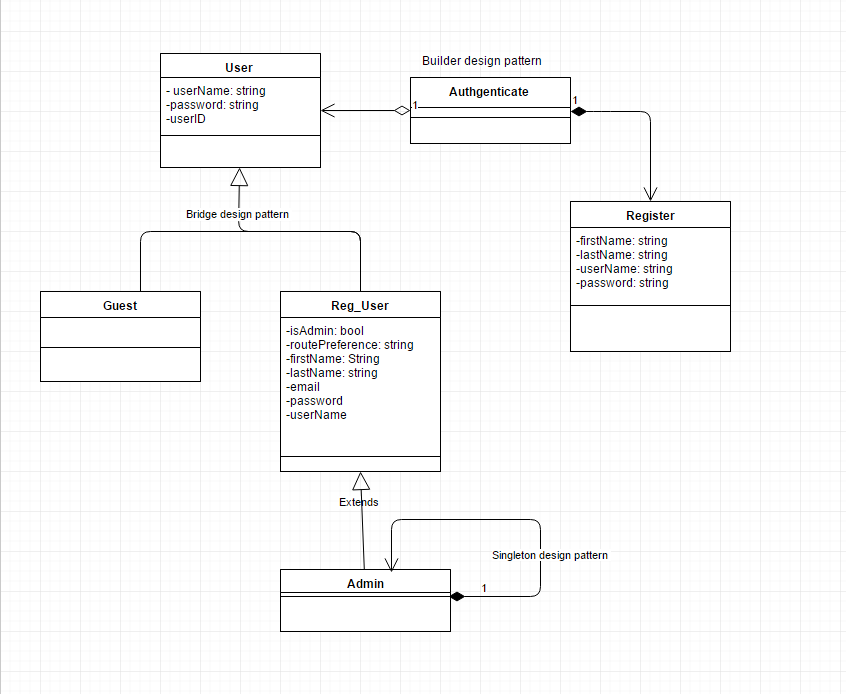
\includegraphics[width=\linewidth,angle=90,scale=1.3]{Images/User_module/UserModuleClassDiagram.png}
        \begin{figure}[h]
            \caption{User Module Class Diagram.}
        \end{figure}
        
\subsection{Use Case Diagram}
        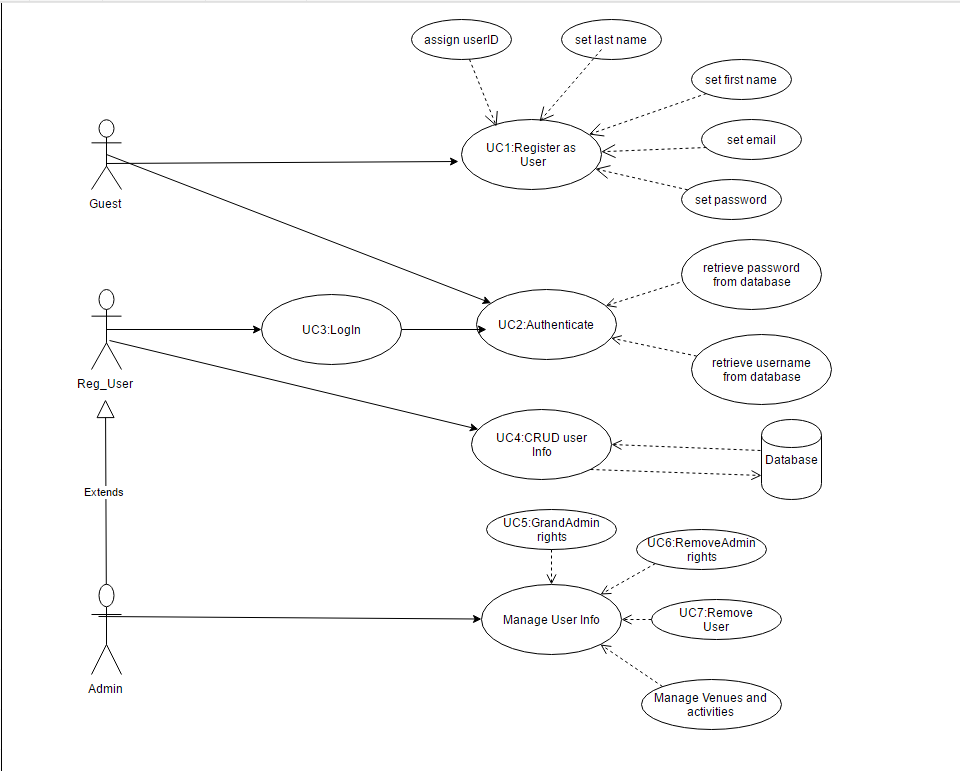
\includegraphics[width=\linewidth,angle=90,scale=1.3]{Images/User_module/UserModuleUsecaseDiagram.png}
        \begin{figure}[h]
            \caption{User Module Use Case Diagram.}
        \end{figure}
        
\end{center}

        
\section{Fitness}
The Fitness module is a nice non-essential addition to the NavUP system that allows the user to track their fitness goals while they're navigating campus. 

\subsection{Design Constraints}
\begin{itemize}

      \item Given that a device does has an accelerometer, the device manufacturer must provide a software interface to interact with the device's accelerometer.
      \item Not all devices models are made equal. Some older devices do not have accelerometers to track steps with. The accuracy of accelerometers also vary from different device manufacturers.
      \item To track steps continuously with a background process will greatly impact the battery life of devices with small battery capacities.
      
\end{itemize}


\subsection{Technology Choices}
There are multiple fitness APIs available for both Android as well as iOS devices. Google Fit is one of such APIs and fulfills the basic requirements for the NavUP Fitness module. It encapsulates a sensors API that provides access to raw data created by various sensors in the android device such as the accelerometer. We will then be able to use this data to track the user's movements and record their number of steps. Similar APIs are available for iOS such as HealthKit.


\subsection{Class Diagram}
        \includegraphics[width=\linewidth,scale=1.5]{Images/Fitness_Module/FitnessClassDiagram.png}
        \begin{figure}[h]
            \caption{Fitness Module Class Diagram.}
        \end{figure}
        
\subsection{Sequence Diagram}
        \includegraphics[width=\linewidth,scale=3]{Images/Fitness_Module/Fitness_Sequence_Diagram.png}
        \begin{figure}[h]
            \caption{Fitness Module Sequence Diagram.}
        \end{figure}










        
        
        
        
        
\begin{center}
\section{System Deployment Diagram}
        \includegraphics[width=\linewidth,angle=90,scale=1.40]{Images/DeploymentDiagram.png}
        \begin{figure}[h]
            \caption{System Deployment Diagram.}
        \end{figure}
        
\end{center}
        

\end{document}
